% State diagram of one jack's JackMonitor (topology/src/monitor.rs): plug detection, identification
% and following, plus the output pipeline of expression_controller.rs.
%
% Build (TeX Live):  pdflatex jack-monitor-states.tex
%   SVG for PowerPoint:  pdftocairo -svg jack-monitor-states.pdf jack-monitor-states.svg
%   PNG fallback:        pdftocairo -png -r 600 -singlefile jack-monitor-states.pdf jack-monitor-states
% In a LaTeX report, 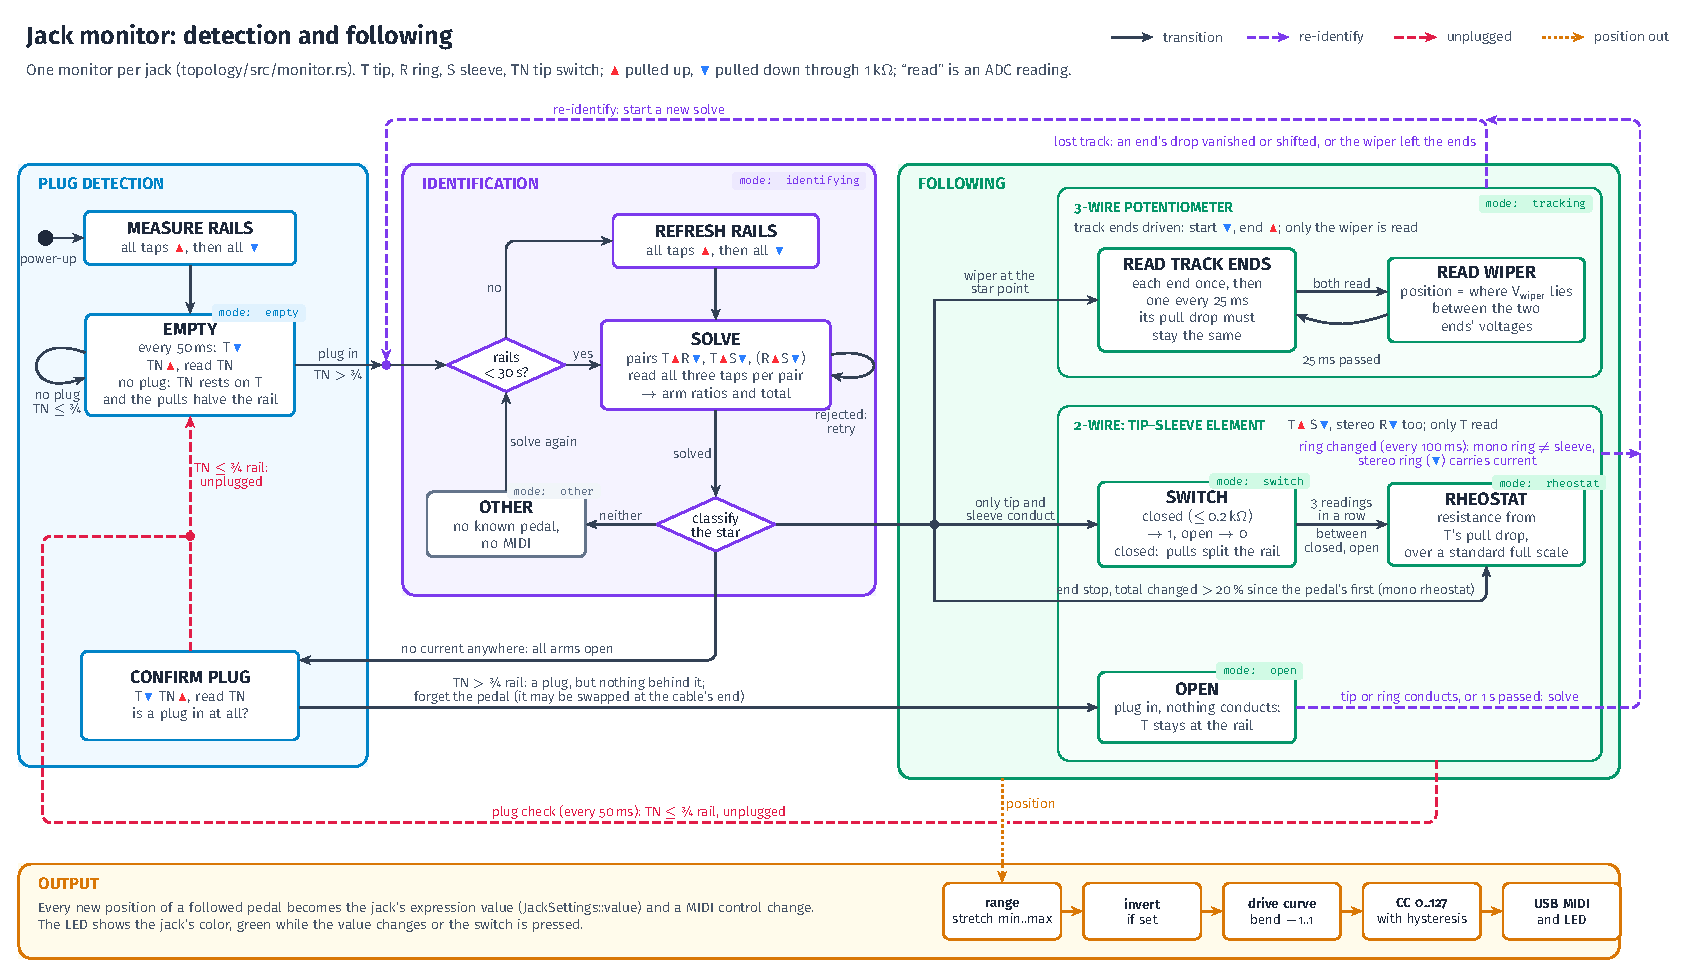
\includegraphics[width=\linewidth]{jack-monitor-states.pdf}.
%
% Layout: three columns read left to right - plug detection, identification, following - on a
% 16:9 canvas. Return edges run in two corridors so they never cross the main flow: re-identifying
% along the top, unplugging along the bottom. The output pipeline sits below everything.

\documentclass[tikz, border=8pt]{standalone}
\usepackage{lmodern}
\usepackage[sfdefault, book]{FiraSans}
\usepackage[scale=0.9]{FiraMono}
\usepackage[T1]{fontenc}
\usepackage{amssymb}
\usetikzlibrary{arrows.meta, positioning, calc, shapes.geometric}

% Tailwind palette: one hue per group, the rails in the web interface's red and blue.
\definecolor{detect}{HTML}{0284C7}      \definecolor{detectFill}{HTML}{F0F9FF}  \definecolor{detectTint}{HTML}{E0F2FE}
\definecolor{ident}{HTML}{7C3AED}       \definecolor{identFill}{HTML}{F5F3FF}   \definecolor{identTint}{HTML}{EDE9FE}
\definecolor{follow}{HTML}{059669}      \definecolor{followFill}{HTML}{ECFDF5}  \definecolor{followTint}{HTML}{D1FAE5}
\definecolor{output}{HTML}{D97706}      \definecolor{outputFill}{HTML}{FFFBEB}  \definecolor{outputTint}{HTML}{FEF3C7}
\definecolor{unplug}{HTML}{E11D48}
\definecolor{other}{HTML}{64748B}       \definecolor{otherTint}{HTML}{F1F5F9}
\definecolor{ink}{HTML}{1E293B}
\definecolor{muted}{HTML}{475569}
\definecolor{wire}{HTML}{334155}
\definecolor{railHigh}{HTML}{FB2C36}
\definecolor{railLow}{HTML}{2B7FFF}

% Drives: a contact pulled up or down through its 1 kOhm pull.
\newcommand{\hi}[1]{#1\kern0.5pt{\color{railHigh}$\blacktriangle$}}
\newcommand{\lo}[1]{#1\kern0.5pt{\color{railLow}$\blacktriangledown$}}
% A state's name and its description lines.
\newcommand{\st}[1]{{\bfseries\fontsize{8.6}{10.5}\selectfont\color{ink}#1}}
\newcommand{\sd}[1]{#1}

\tikzset{
  >={Stealth[length=5pt, width=4pt]},
  every node/.style={text=ink},
  group/.style={draw=#1, line width=0.9pt, rounded corners=6pt},
  groupTitle/.style={anchor=north west, font=\bfseries\footnotesize, text=#1},
  subgroup/.style={draw=#1, line width=0.6pt, rounded corners=5pt, fill=white, fill opacity=0.55},
  subgroupTitle/.style={anchor=north west, font=\bfseries\scriptsize, text=#1},
  info/.style={anchor=north west, font=\fontsize{6.6}{8}\selectfont, text=muted},
  state/.style={draw=#1, fill=white, line width=0.9pt, rounded corners=3pt, align=center,
    inner sep=4pt, text width=3.6cm, minimum height=1.1cm,
    font=\fontsize{6.8}{8.4}\selectfont, text=muted},
  decision/.style={draw=#1, fill=white, line width=0.9pt, diamond, aspect=2.2, inner sep=1pt,
    align=center, font=\fontsize{6.8}{8}\selectfont},
  chip/.style={fill=#1, rounded corners=2pt, inner xsep=3pt, inner ysep=1.5pt,
    font=\ttfamily\fontsize{6}{7}\selectfont},
  trans/.style={->, line width=0.8pt, draw=wire, rounded corners=4pt},
  reident/.style={->, line width=0.9pt, draw=ident, dashed, dash pattern=on 4pt off 2pt, rounded corners=4pt},
  unplugged/.style={->, line width=0.9pt, draw=unplug, dashed, dash pattern=on 4pt off 2pt, rounded corners=4pt},
  feed/.style={->, line width=0.9pt, draw=output, dash pattern=on 1.2pt off 1.6pt, rounded corners=4pt},
  lbl/.style={font=\fontsize{6.4}{7.6}\selectfont, text=muted, align=center, inner sep=1.5pt},
  junction/.style={circle, fill=#1, inner sep=0pt, minimum size=4pt},
  box/.style={draw=output, fill=white, line width=0.8pt, rounded corners=3pt, align=center,
    text width=1.85cm, minimum height=0.95cm, inner sep=2pt, font=\fontsize{6.4}{7.6}\selectfont},
}

\begin{document}
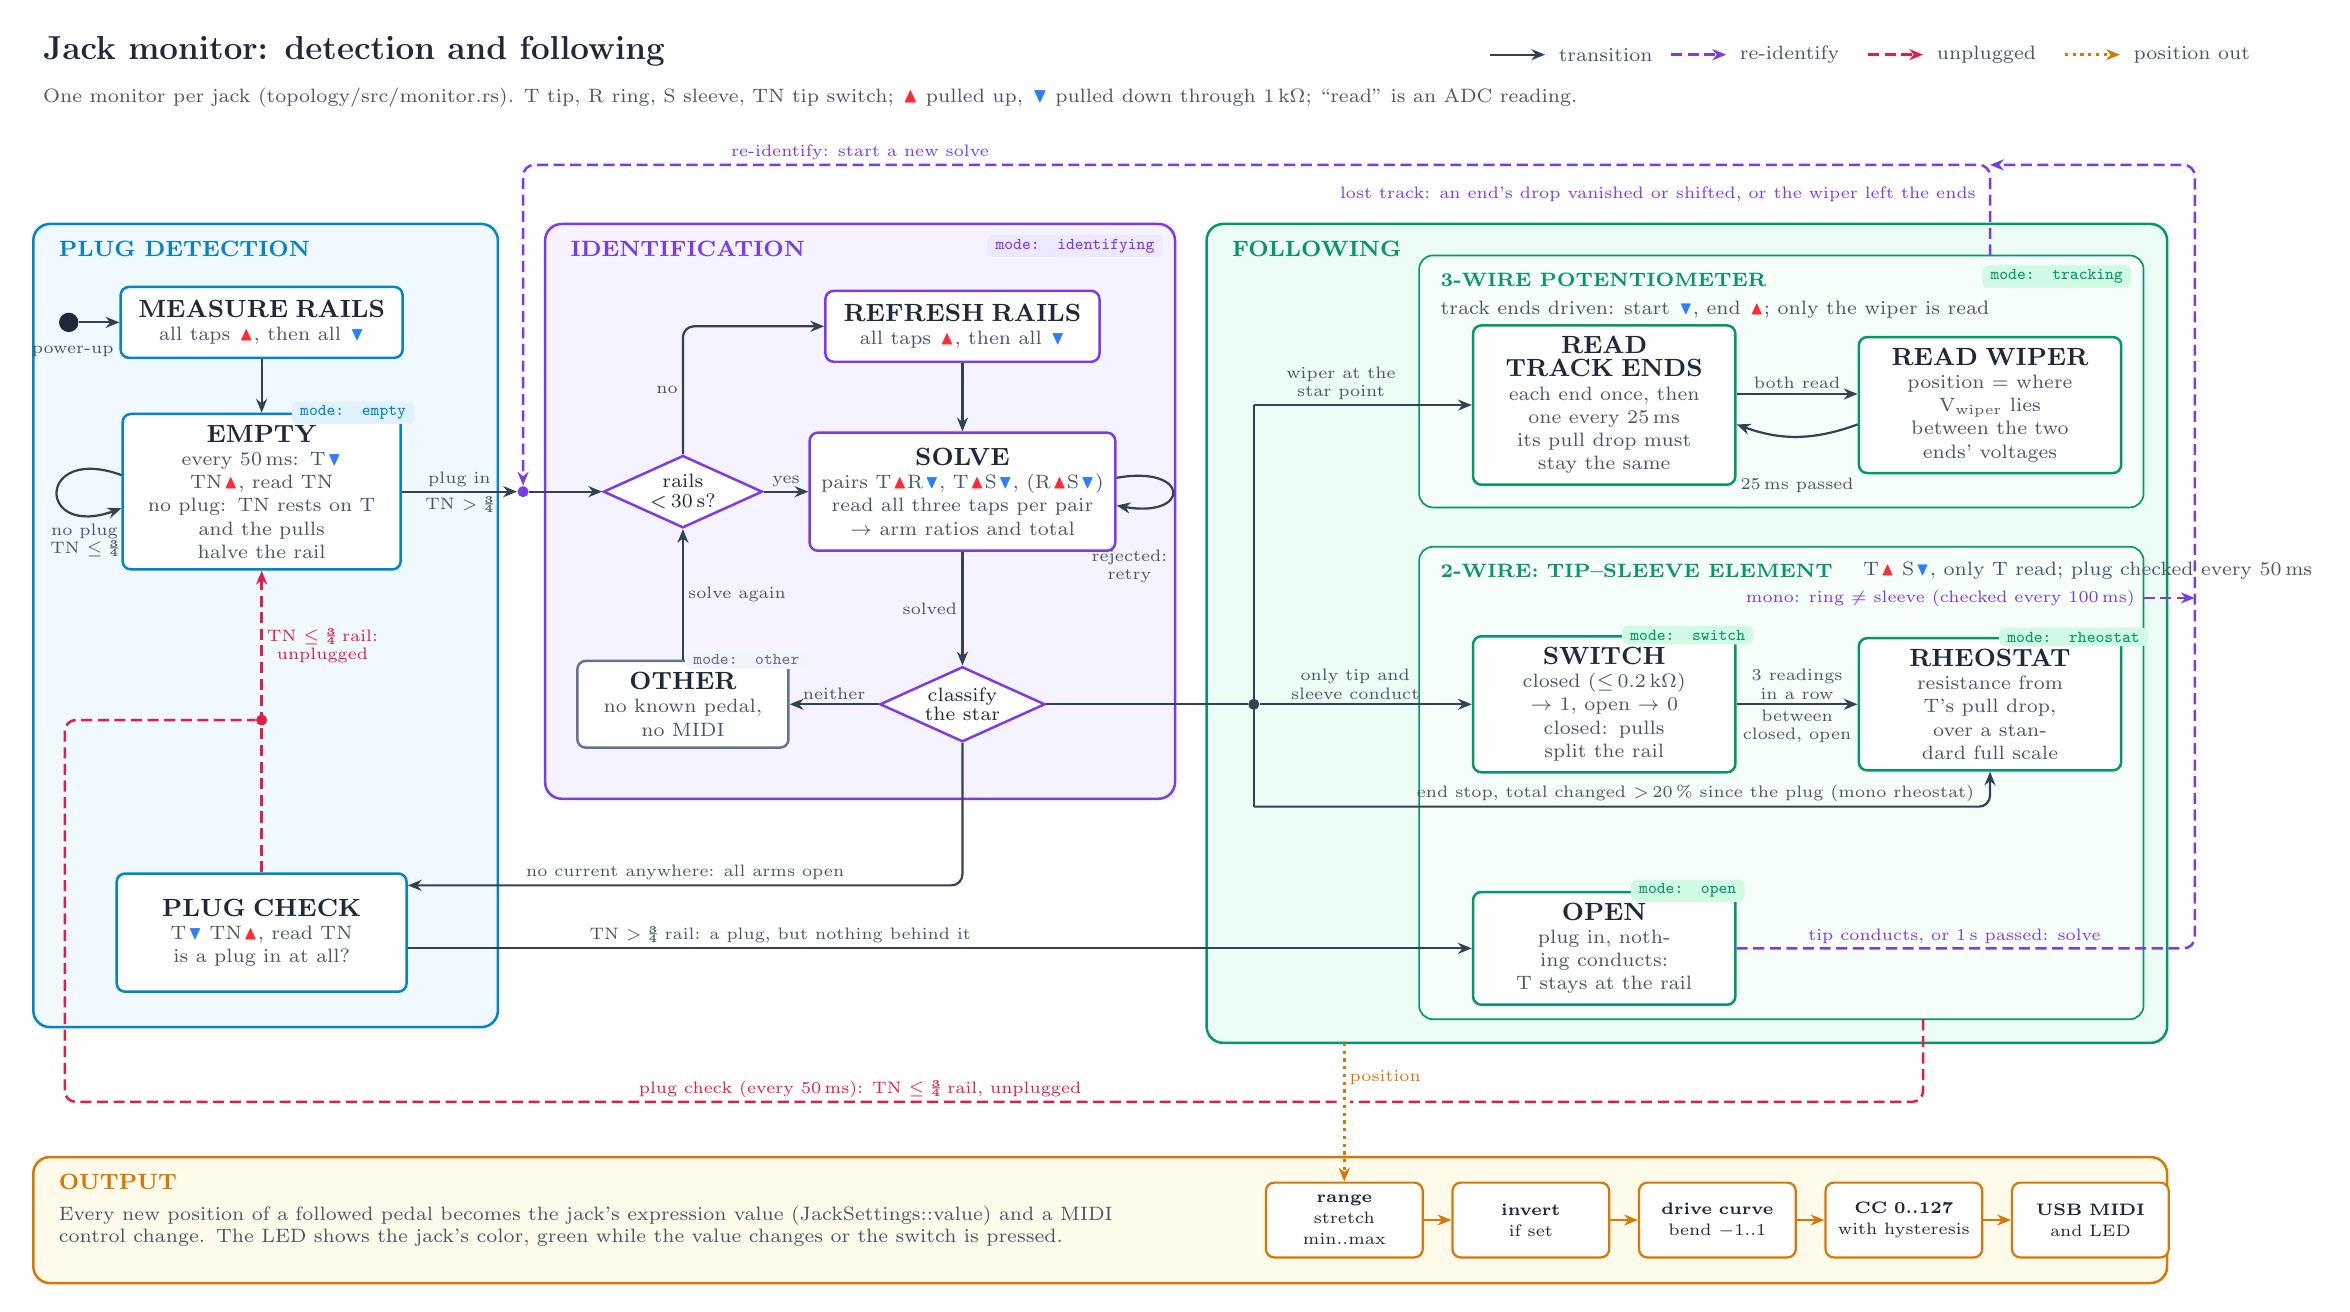
\begin{tikzpicture}

  % ---------------------------------------------------------------- title and legend
  \node[anchor=north west, font=\bfseries\large] at (0.5, 16.1) {Jack monitor: detection and following};
  \node[anchor=north west, font=\fontsize{7.4}{9}\selectfont, text=muted] at (0.5, 15.45)
    {One monitor per jack (topology/src/monitor.rs).
     T tip, R ring, S sleeve, TN tip switch;
     \hi{} pulled up, \lo{} pulled down through 1\,k$\Omega$; ``read'' is an ADC reading.};

  \begin{scope}[shift={(19.0, 15.75)}, font=\fontsize{6.6}{8}\selectfont]
    \draw[trans] (0, 0) -- (0.7, 0);        \node[anchor=west, text=muted] at (0.75, 0) {transition};
    \draw[reident] (2.3, 0) -- (3.0, 0);    \node[anchor=west, text=muted] at (3.05, 0) {re-identify};
    \draw[unplugged] (4.8, 0) -- (5.5, 0);  \node[anchor=west, text=muted] at (5.55, 0) {unplugged};
    \draw[feed] (7.3, 0) -- (8.0, 0);       \node[anchor=west, text=muted] at (8.05, 0) {position out};
  \end{scope}

  % ---------------------------------------------------------------- groups
  \fill[detectFill] (0.5, 3.4) rectangle (6.4, 13.6);
  \draw[group=detect] (0.5, 3.4) rectangle (6.4, 13.6);
  \node[groupTitle=detect] at (0.7, 13.5) {PLUG DETECTION};

  \fill[identFill] (7.0, 6.3) rectangle (15.0, 13.6);
  \draw[group=ident] (7.0, 6.3) rectangle (15.0, 13.6);
  \node[groupTitle=ident] at (7.2, 13.5) {IDENTIFICATION};
  \node[chip=identTint, text=ident, anchor=north east] at (14.85, 13.47) {mode: identifying};

  \fill[followFill] (15.4, 3.2) rectangle (27.6, 13.6);
  \draw[group=follow] (15.4, 3.2) rectangle (27.6, 13.6);
  \node[groupTitle=follow] at (15.6, 13.5) {FOLLOWING};

  \draw[subgroup=follow] (18.1, 10.0) rectangle (27.3, 13.2);
  \node[subgroupTitle=follow] at (18.25, 13.1) {3-WIRE POTENTIOMETER};
  \node[info] at (18.25, 12.75) {track ends driven: start \lo{}, end \hi{}; only the wiper is read};
  \node[chip=followTint, text=follow, anchor=north east] at (27.15, 13.08) {mode: tracking};

  \draw[subgroup=follow] (18.1, 3.5) rectangle (27.3, 9.5);
  \node[subgroupTitle=follow] (twoWire) at (18.25, 9.4) {2-WIRE: TIP--SLEEVE ELEMENT};
  \node[info, anchor=west] at ([xshift=4pt]twoWire.east) {\hi{T} \lo{S}, only T read; plug checked every 50\,ms};

  % ---------------------------------------------------------------- plug detection
  \node[circle, fill=ink, minimum size=7pt, inner sep=0pt] (start) at (0.95, 12.35) {};
  \node[lbl, anchor=north] at (1.0, 12.1) {power-up};
  \node[state=detect, text width=3.3cm, minimum height=0.9cm] (rails) at (3.4, 12.35)
    {\st{MEASURE RAILS}\\ \sd{all taps \hi{}, then all \lo{}}};
  \draw[trans] (start) -- (rails);

  \node[state=detect, text width=3.25cm, minimum height=1.6cm] (empty) at (3.4, 10.2)
    {\st{EMPTY}\\ \sd{every 50\,ms: \lo{T} \hi{TN}, read TN}\\ \sd{no plug: TN rests on T}\\ \sd{and the pulls halve the rail}};
  \node[chip=detectTint, text=detect, anchor=center] at ($(empty.north east)+(-0.62,0)$) {mode: empty};
  \draw[trans] (rails.south) -- (rails.south |- empty.north);
  \draw[trans] ([yshift=6pt]empty.west) to[out=160, in=200, looseness=7] ([yshift=-6pt]empty.west);
  \node[lbl, anchor=north] at (1.15, 9.85) {no plug\\[-1pt]TN $\leq$ \textthreequarters};

  \node[state=detect, text width=3.4cm, minimum height=1.5cm] (plugcheck) at (3.4, 4.6)
    {\st{PLUG CHECK}\\ \sd{\lo{T} \hi{TN}, read TN}\\ \sd{is a plug in at all?}};
  \draw[unplugged] (plugcheck.north) -- (empty.south)
    node[lbl, pos=0.75, right, text=unplug] {TN $\leq$ \textthreequarters{} rail:\\[-1pt]unplugged};

  % ---------------------------------------------------------------- identification
  \node[junction=ident] (entry) at (6.72, 10.2) {};
  \draw[trans] (empty.east) -- (entry) node[lbl, midway, above] {plug in} node[lbl, midway, below] {TN $>$ \textthreequarters{}};
  \node[decision=ident] (fresh) at (8.75, 10.2) {rails\\[-1pt]$<$\,30\,s?};
  \draw[trans] (entry) -- (fresh);

  \node[state=ident, text width=3.2cm, minimum height=0.9cm] (refresh) at (12.3, 12.3)
    {\st{REFRESH RAILS}\\ \sd{all taps \hi{}, then all \lo{}}};
  \draw[trans] (fresh.north) |- (refresh.west) node[lbl, pos=0.25, left] {no};

  \node[state=ident, text width=3.6cm, minimum height=1.5cm] (solve) at (12.3, 10.2)
    {\st{SOLVE}\\ \sd{pairs \hi{T}\lo{R}, \hi{T}\lo{S}, (\hi{R}\lo{S})}\\ \sd{read all three taps per pair}\\ \sd{$\rightarrow$ arm ratios and total}};
  \draw[trans] (fresh.east) -- (solve.west) node[lbl, midway, above] {yes};
  \draw[trans] (refresh.south) -- (solve.north);
  \draw[trans] ([yshift=5pt]solve.east) to[out=10, in=-10, looseness=7] ([yshift=-5pt]solve.east);
  \node[lbl, anchor=north] at (14.42, 9.52) {rejected:\\[-1pt]retry};

  \node[decision=ident] (classify) at (12.3, 7.5) {classify\\[-1pt]the star};
  \draw[trans] (solve.south) -- (classify.north) node[lbl, midway, left] {solved};

  \node[state=other, text width=2.4cm, minimum height=1.1cm] (other) at (8.75, 7.5)
    {\st{OTHER}\\ \sd{no known pedal,}\\ \sd{no MIDI}};
  \node[chip=otherTint, text=other, anchor=center] at ($(other.north east)+(-0.55,0)$) {mode: other};
  \draw[trans] (classify.west) -- (other.east) node[lbl, midway, above] {neither};
  \draw[trans] (other.north) -- (fresh.south) node[lbl, midway, right] {solve again};

  \draw[trans] (classify.south) |- (plugcheck.east |- 0, 5.2)
    node[lbl, pos=0.75, above] {no current anywhere: all arms open};

  % ---------------------------------------------------------------- following: distribution
  \node[junction=wire] (split) at (16.0, 7.5) {};
  \draw[line width=0.8pt, draw=wire] (classify.east) -- (split);
  \draw[line width=0.8pt, draw=wire, rounded corners=4pt] (16.0, 11.3) -- (16.0, 6.2);

  % ---------------------------------------------------------------- following: tracking
  \node[state=follow, text width=3.05cm, minimum height=1.25cm] (ends) at (20.45, 11.3)
    {\st{READ TRACK ENDS}\\ \sd{each end once, then one every 25\,ms}\\ \sd{its pull drop must stay the same}};
  \node[state=follow, text width=3.05cm, minimum height=1.25cm] (wiper) at (25.35, 11.3)
    {\st{READ WIPER}\\ \sd{position = where V\textsubscript{wiper} lies}\\ \sd{between the two ends' voltages}};
  \draw[trans] (16.0, 11.3) -- (ends.west)
    node[lbl, pos=0.4, above] {wiper at the\\[-1pt]star point};
  \draw[trans] ([yshift=4pt]ends.east) -- ([yshift=4pt]wiper.west) node[lbl, midway, above] {both read};
  \draw[trans] ([yshift=-7pt]wiper.west) to[out=200, in=-20] ([yshift=-7pt]ends.east);
  \node[lbl] at (22.9, 10.28) {25\,ms passed};

  % ---------------------------------------------------------------- following: tip-sleeve
  \node[state=follow, text width=3.05cm, minimum height=1.2cm] (switch) at (20.45, 7.5)
    {\st{SWITCH}\\ \sd{closed ($\leq$\,0.2\,k$\Omega$) $\rightarrow$ 1, open $\rightarrow$ 0}\\ \sd{closed: pulls split the rail}};
  \node[chip=followTint, text=follow, anchor=center] at ($(switch.north east)+(-0.62,0)$) {mode: switch};
  \node[state=follow, text width=3.05cm, minimum height=1.2cm] (rheostat) at (25.35, 7.5)
    {\st{RHEOSTAT}\\ \sd{resistance from T's pull drop,}\\ \sd{over a standard full scale}};
  \node[chip=followTint, text=follow, anchor=center] at ($(rheostat.north east)+(-0.62,0)$) {mode: rheostat};
  \node[state=follow, text width=3.05cm, minimum height=1.2cm] (open) at (20.45, 4.4)
    {\st{OPEN}\\ \sd{plug in, nothing conducts:}\\ \sd{T stays at the rail}};
  \node[chip=followTint, text=follow, anchor=center] at ($(open.north east)+(-0.62,0)$) {mode: open};

  \draw[trans] (split) -- (switch.west) node[lbl, pos=0.45, above] {only tip and\\[-1pt]sleeve conduct};
  \draw[trans] (16.0, 6.2) -| (rheostat.south)
    node[lbl, pos=0.3, above] {end stop, total changed $>$\,20\,\% since the plug (mono rheostat)};
  \draw[trans] (switch.east) -- (rheostat.west)
    node[lbl, midway, above] {3 readings\\[-1pt]in a row}
    node[lbl, midway, below] {between\\[-1pt]closed, open};
  \draw[trans] (plugcheck.east |- 0, 4.4) -- (open.west)
    node[lbl, pos=0.35, above] {TN $>$ \textthreequarters{} rail: a plug, but nothing behind it};

  % ---------------------------------------------------------------- return corridors
  % Re-identify: along the top into the identification entry.
  \draw[reident] (wiper.north |- 0, 13.2) -- (wiper.north |- 0, 14.35) -- (6.72, 14.35) -- (entry);
  \node[lbl, anchor=east, text=ident] at ($(wiper.north |- 0, 13.97)+(-0.12, 0)$)
    {lost track: an end's drop vanished or shifted, or the wiper left the ends};
  \draw[reident] (open.east) -- (27.95, 4.4) -- (27.95, 14.35) -- (wiper.north |- 0, 14.35);
  \node[lbl, text=ident, anchor=south] at (24.9, 4.4) {tip conducts, or 1\,s passed: solve};
  \draw[reident] (27.3, 8.85) -- (27.95, 8.85);
  \node[lbl, text=ident, anchor=east] at (27.25, 8.85) {mono: ring $\neq$ sleeve (checked every 100\,ms)};
  \node[lbl, text=ident, anchor=south] at (11.0, 14.35) {re-identify: start a new solve};

  % Unplugged: along the bottom into EMPTY.
  \node[junction=unplug] (unplugMerge) at (plugcheck.north |- 0, 7.3) {};
  \draw[unplugged, -] (24.5, 3.5) -- (24.5, 2.45) -- (0.9, 2.45) -- (0.9, 7.3) -- (unplugMerge);
  \node[lbl, text=unplug, anchor=south] at (11.0, 2.45) {plug check (every 50\,ms): TN $\leq$ \textthreequarters{} rail, unplugged};

  % ---------------------------------------------------------------- output pipeline
  \fill[outputFill] (0.5, 0.15) rectangle (27.6, 1.75);
  \draw[group=output] (0.5, 0.15) rectangle (27.6, 1.75);
  \node[groupTitle=output] at (0.7, 1.65) {OUTPUT};
  \node[info, text width=13.6cm] at (0.7, 1.25)
    {Every new position of a followed pedal becomes the jack's expression value
     (JackSettings::value) and a MIDI control change. The LED shows the jack's color,
     green while the value changes or the switch is pressed.};

  \node[box] (range) at (17.15, 0.95) {\textbf{range}\\ stretch min..max};
  \node[box, right=0.35cm of range] (invert) {\textbf{invert}\\ if set};
  \node[box, right=0.35cm of invert] (drive) {\textbf{drive curve}\\ bend $-$1..1};
  \node[box, right=0.35cm of drive] (cc) {\textbf{CC 0..127}\\ with hysteresis};
  \node[box, right=0.35cm of cc] (usb) {\textbf{USB MIDI}\\ and LED};
  \foreach \from/\to in {range/invert, invert/drive, drive/cc, cc/usb}
    \draw[->, line width=0.8pt, draw=output] (\from) -- (\to);

  % Position out of the following group, bridging the unplug corridor.
  \draw[white, line width=4pt] (17.15, 2.2) -- (17.15, 2.7);
  \draw[feed] (17.15, 3.2) -- (range.north) node[lbl, pos=0.25, right, text=output] {position};

\end{tikzpicture}
\end{document}
